\documentclass[a4paper]{article}
\usepackage[utf8]{inputenc}
\usepackage[russian]{babel}
\usepackage[T2]{fontenc}
\usepackage[warn]{mathtext}
\usepackage{caption}

\usepackage{graphicx}
\graphicspath{ {images/} }
\usepackage{tikz}
\usepackage{pgfplots}

\usepackage{amsmath}
\usepackage{floatflt}
\usepackage[left=20mm, top=20mm, right=20mm, bottom=20mm, footskip=10mm]{geometry}

\usepackage{multicol}
\setlength{\columnsep}{2cm}


\usepackage{multicol}
\setlength{\columnsep}{2cm}
\begin{document}
	
\begin{titlepage}
	\centering
	\vspace{5cm}
	{\scshape\LARGE Московский физико-технический институт \par}
	\vspace{4cm}
	{\scshape\Large Лабораторная работа 4.3.1 \par}
	\vspace{1cm}
	{\huge\bfseries Диффракция. \par}
	\vspace{1cm}
	\vfill
\begin{flushright}
	{\large выполнил студент 924 группы ФОПФ}\par
	\vspace{0.3cm}
	{\LARGE Панферов Андрей}
\end{flushright}
	

	\vfill

% Bottom of the page
	Долгопрудный, 2021 г.
\end{titlepage}

\paragraph*{Цель работы:} Исследовать явления дифракции Френеля и Фраунгофера на щели, изучить влияние дифракции на разрешающую способность оптических приборов.
	
\paragraph*{Оборудование:} 
\begin{itemize}
    \item оптическая скамья
    \item ртутная лампа
    \item монохроматор
    \item щели с регулируемой шириной
    \item рамка с вертикальной нитью
    \item двойная щель
    \item микроскоп на поперечных салазках с микрометрическим винтом
    \item зрительная труба
\end{itemize}

\section*{Дифракция Френеля на щели}
\begin{enumerate}
    \item Соберем установку для наблюдения дифракции Френеля на щели, представленную на рис.\ref{fig:fren}. Дифракционная картина рассматривается с помощью микроскопа М, сфокусированного на некую плоскость наблюдения П. 
\begin{figure}[h]
    \centering
    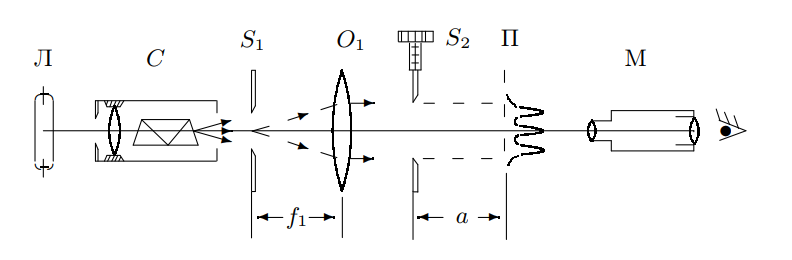
\includegraphics[width=15cm]{setup_frenel.PNG}
    \caption{Схема лабораторной установки для наблюдения дифракции Френеля}
    \label{fig:fren}
\end{figure}

\item Измерим ширину $b$ щели $S_2$ с помощью микрометрического винта и поперечных салазок микроскопа и 
\[b_{micro} = (2,740 \pm 0,005) \cdot 10^{-4} \text{м}\]
\[b_{shel} = (3,00 \pm 0,05) \cdot 10^{-4} \text{м}\]
В данных, написанных выше, берем погрешность, равную половине цены деления шкалы, то есть в случае микрометрического винта: $0,001/2$, а в случае салазок микроскопа: $0,01/2$.

\item Снимем зависимость координаты микроскопа от числа наблюдаемых полос, результаты занесём в таблицу 1.


\begin{table}[h]
    \centering
    \begin{center}
    \caption{Количество минимумов в зависимости от расстояния до плоскости наблюдения}
    \end{center}
    \vspace{0.1cm}
    \label{fren_data}
    \begin{tabular}{ |p{2.5cm}||p{0.5cm}|p{0.5cm}|p{0.5cm}|p{0.5cm}|p{0.5cm}|p{0.5cm}|p{0.5cm}|p{0.5cm}|}
 \hline
n тёмных полос & 0 & 1 & 2 & 3 & 4 & 5\\
 \hline
 $z$, мм & 481 & 475 & 467 & 462 & 460 & 459 \\
 \hline
 $a$, мм & 28 & 22 & 14 & 9 & 7 & 6 \\
 \hline
 $\xi$, мкм & - & 110 & 124 & 121 & 124 & 128 \\ 
 \hline
 
\end{tabular}
\end{table}


\item Сравним размер зон Френеля с измеренной шириной $b = 300$ мкм щели $S_2$. Для этого рассчитаем величину $\xi_n=\sqrt{an\lambda}$ ($\lambda = 546.1$ нм) и построим график зависимости $\xi(n)$ и нанесем на него прямую $y = b/2$

\begin{center}
    \begin{tikzpicture}[scale=1]
        	\begin{axis}[
        		axis lines = middle,
            	xlabel = {$n$},
            	ylabel = {$2\xi$},
            	ylabel style={red, scale=1},
            	xlabel style={red, scale=1},
            	ymin = 0,
            	title={Зависимость $\xi(n)$},
            	table/col sep=semicolon,
        		]
        		\addplot +[blue, only marks] table[x=n, y=xi]{Fren.csv};
        		\addplot[color=red, domain=0:5]{137};
        	\end{axis}
        \end{tikzpicture}
    \end{center}

Видим, что ширина френелевских зон - величина порядка толщины щели.

\item Пронаблюдаем за дифракцией Френеля на проволоке. При удалении микроскопа от нити на её фоне всегда наблюдается чётное число тёмных дифракционных полос (светлый центр).

\end{enumerate}

\section*{Дифракция Фраунгофера на щели}

На значительном удалении от щели, когда ширина щели становится значительно меньше ширины первой зоны Френеля, изображение щели размывается и возникает дифракционная картина, называемая дифракцией Фраунгофера.

\begin{enumerate}
    \item Дифракцию Френеля и Фраунгофера можно наблюдать на одной и той же установке (поставив дополнительную линзу между щелью и плоскостью наблюдения). Дифракционная картина наблюдается в фокальной плоскости объектива $O_2$ (фокусное расстояние линзы $f_2 = 12.8$ см). Схема установки для наблюдения дифракции Фраунгофера на щели представлена на рис. 6. Фотография дифракционной картинцы представлена на рис. 8.
    
  \begin{figure}[h]
    \centering
    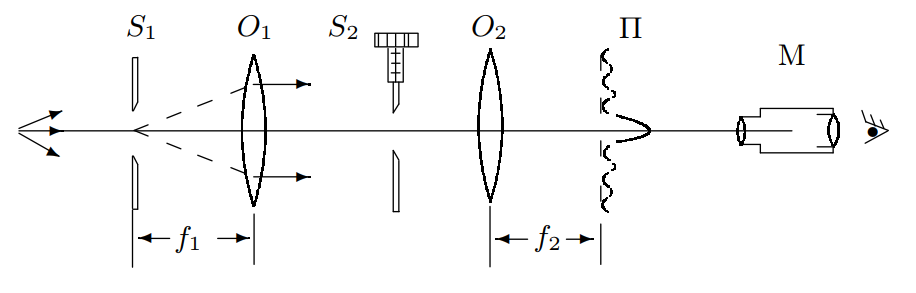
\includegraphics[width=12cm]{setup_fraunhofer.PNG}
    \caption{Схема лабораторной установки для наблюдения дифракции Фраунгофера на щели}
    \label{fig:fraun}
\end{figure}  
    
    \item Настроим установку, с помощью винта поперечного перемещения микроскопа измерим координаты $X_m$ нескольких дифракционных минимумов от $-m$ до $m$. Занесём результаты в таблицу 2 (цена деления шкалы - 0.02 мм). 
    
    \begin{table}[h]
    \centering
    \begin{center}
    \caption{Координаты минимумов дифракционной картины}
    \end{center}
    \vspace{0.1cm}
    \label{tab:fraun}
    \begin{tabular}{|l|c|c|c|c|c|c|c|c|c|}
 \hline
m & -4 & -3 & -2 & -1 & 0 & 1 & 2 & 3 & 4 \\
 \hline
 Дел. & -58 & -43 & -29 & -15 & 0 & 15 & 29 & 43 & 58 \\
 $x$, мм & -1.16 & -0.86 & -0.58 & -0.30 & 0 & 0.30 & 0.58 & 0.86 & 1.16 \\

 \hline
 
\end{tabular}
\end{table}

\item Построим график зависимости $x(m)$. По угловому коэффициенту $k = (0.289 \pm 0.005)$мм прямой определим среднее расстояние между соседними минимумами, рассчитаем ширину щели по формуле $b = \frac{\lambda f_2}{k} = 242$ мкм. Это значение практически совпадает с измеренным по микрометрическому винту ($b_0 = 223$ мкм)

\begin{center}
    \begin{tikzpicture}[scale=1]
        \begin{axis}[
            	axis lines = middle,
            	xlabel = {m},
                ylabel = {x, мм},
            	ylabel style={red, scale=1},
                xlabel style={red, scale=1},
            	title={Зависимость x(m)},
            	table/col sep=semicolon,
            ]
    	    \addplot +[blue, only marks] table[x=m, y=x]{Fraun.csv};
    	    \addplot[color=red]{0.29 * x};
    	\end{axis}
    \end{tikzpicture}
\end{center}

\end{enumerate}

\section*{Дифракция Фраунгофера на двух щелях}

\begin{enumerate}
     \item В установке для дифракции Фраунгофера для одной щели заменяем щель $S_2$ экраном Э с двумя щелями (Рис. 3). В итоге получаем характерное распределение максимумов и минимумов (рис. 4 - дифракционная картина Фраунгофера на двух щелях)

\begin{minipage}{0.5\textwidth}
        \centering
        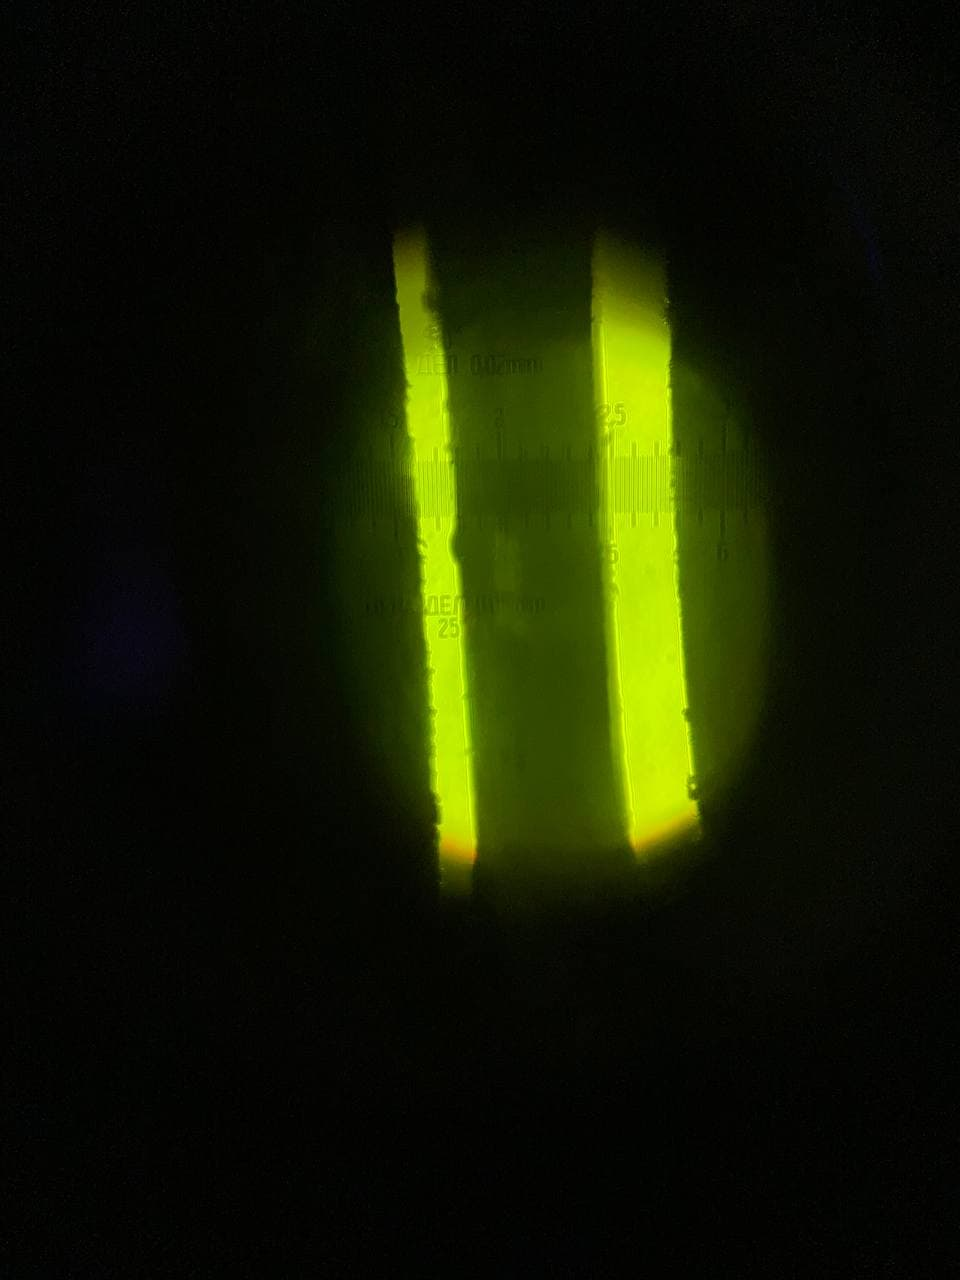
\includegraphics[width=0.8\textwidth]{slit.jpg}
        \captionof{figure}{Фотография щелей в микроскоп}
        \label{fig:slit}
\end{minipage}
\begin{minipage}{0.5\textwidth}
        \centering
        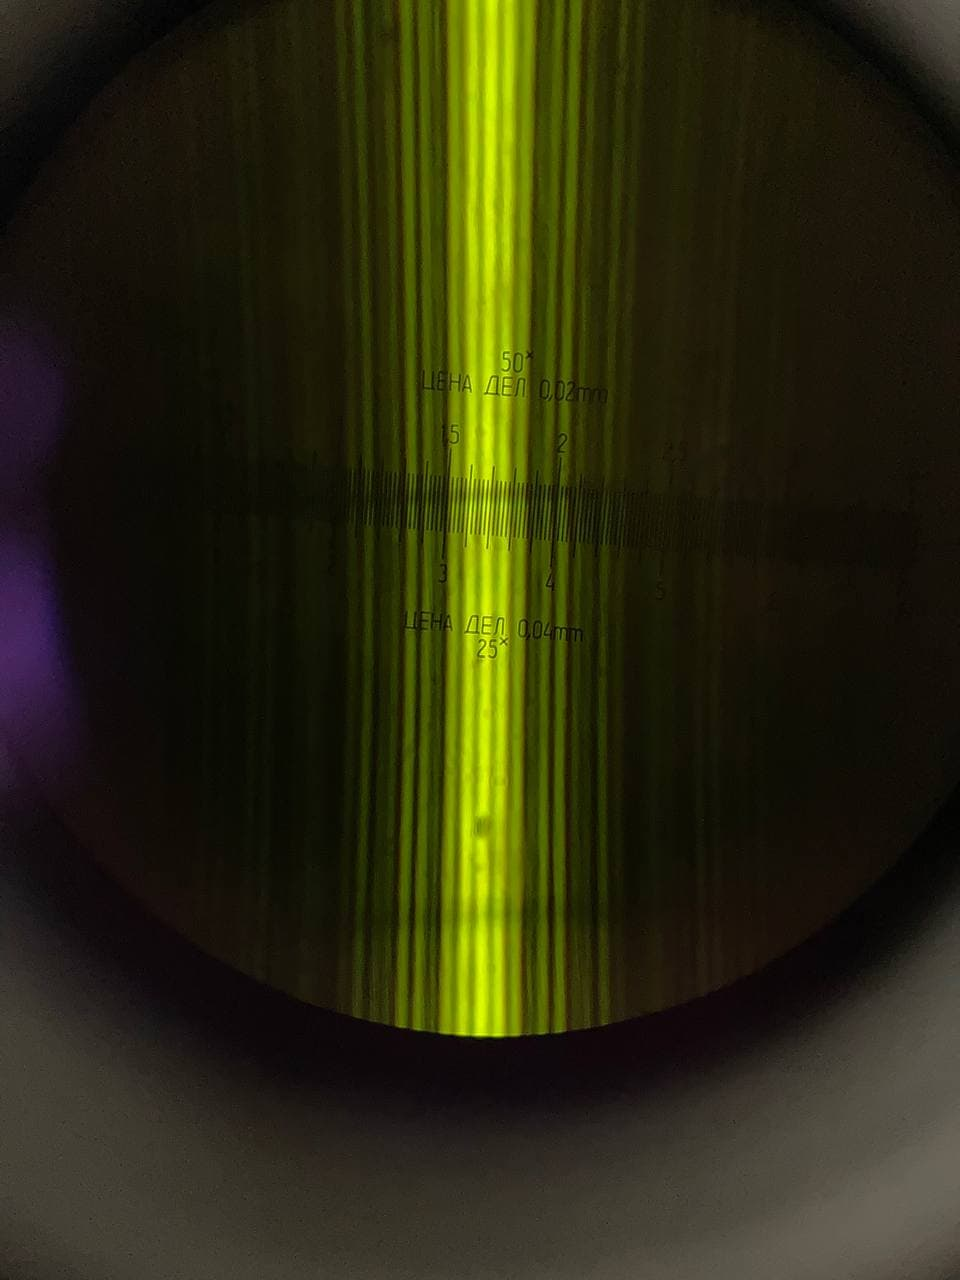
\includegraphics[width=0.8\textwidth]{slit_diff.jpg}
        \captionof{figure}{Дифракционная картина на двух щелях}
        \label{fig:slit_diff}
\end{minipage}
     
\item Определим расстояние между темными полосками внутри центрального максимума. Посчитаем число светлых промежутков между ними. Измерим ширину центрального максимума. $X = (0,44 \pm 0,01)$ мм, между ними $n = 6 \pm 1$ светлых промежутков.

Погрешность для $X$ взялась из половины цены деления, а для $n$ она появилась в связи с тем, что картина полос размыта в области низкой видности.
Далее определим расстояние $\delta x$ между минимумами по формуле $\delta x = \frac{X}{n} = (73 \pm 10)$ мкм. Далее мы можем получить расстояние между щелями $d = \frac{\lambda f_2}{\delta x} = (1.0 \pm 0.2)$мм
\end{enumerate}

\section*{Влияние дифракции на разрешающую способность оптического инструмента}

\begin{figure}[h]
\begin{center}
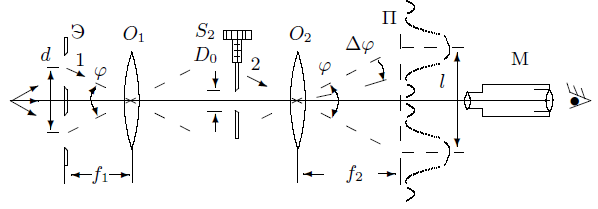
\includegraphics[width = 0.8\textwidth]{degradation.png}
\caption{Схема установки для пункта 4.}
\end{center}
\end{figure}

Если перед $O_2$ расположить $S_2$, то изображение объекта будет искажено из-за дифракции. Качественной характеристикой этого искажения может служить $\varphi_{min}$ --- минимальное угловое между объектами (источниками). 

\begin{equation*}
\varphi = \frac{d}{f_1}
\end{equation*}
Из геометрии $l$ между объектами равно 
\begin{equation*}
l = \phi \cdot d_2
\end{equation*}
\begin{equation*}
\dfrac{\lambda}{b_0} = \dfrac{l}{f_2} = \dfrac{d}{f_1}
\end{equation*}
\begin{enumerate}
\item Собрать схему, изменив в схеме из предыдущего пункта только $S$.
\item Поставить между линзами щель $S_2$ и уменьшая ее ширину наблюдать ухудшение изображения. Подобрать ширину $S_2$ так, чтобы изображения почти сливались.
\[b_0 = (0,093 \pm 0,005)\text{мм}\]


Погрешность берем как половину цены деления.
В итоге получаем, что выполнено соотношение $\frac{\lambda}{b_0} = 5.87 \cdot 10^{-3} \approx \frac{d}{f_1} = 8.7 \cdot 10^{-3}$.
\item Поставить двойную щель и измерить расстояние между щелями и толщину самих щелей.
\begin{align*}
    d_0 &= (0,93 \pm 0,05) \text{мм}\\
    D1 &= (0,18 \pm 0,01) \text{мм}\\
    D2 &= (0,36 \pm 0,01) \text{мм}\\
\end{align*}

\end{enumerate}

\section*{Вывод}

В ходе работы было изучено явление дифракции света - дифракция Френеля на щели и на препятствии, дифракция Фраунгофера на одной и двух щелях.

\begin{itemize}
    \item При исследовании явления дифракции Френеля на щели убедились, что ширина зон Френеля примерно равна ширине щели
    
    \item При исследовании явления дифракции Фраунгофера на щели получили значение ширины щели, примерно равно измеренному непосредственно с помощью регулятора ширины щели:
    \begin{center}
        $b_0 = 223 $мкм \hspace{1cm} $b_f = 242$ мкм
    \end{center}
    
    \item При исследовании явления дифракции Фраунгофера на двух щелях было получено значение расстояния между щелями, примерно равное измеренному с помощью микроскопа:
    
    \begin{center}
        $d_0 = 0.93$ мм \hspace{1cm} $d_f = 1$ мм
    \end{center}
\end{itemize}

\end{document}